% Chương 3 (sửa trực tiếp; bản tiếng Việt)
\chapter{THIẾT KẾ VÀ CÀI ĐẶT HỆ THỐNG}

\section{Kiến trúc}

Hệ thống gồm hai giai đoạn trên cùng một thiết bị. Runtime phát hiện biến khung hình camera thành các bộ khung xương trên Hailo-8, và phần phân tích mức độ tập trung biến các bộ khung xương thành một tỷ lệ ở cấp lớp. Khung hình chỉ tồn tại trong bộ nhớ, và mặc định trạng thái của từng học sinh không bao giờ được xuất ra.

\begin{figure}[H]
\centering
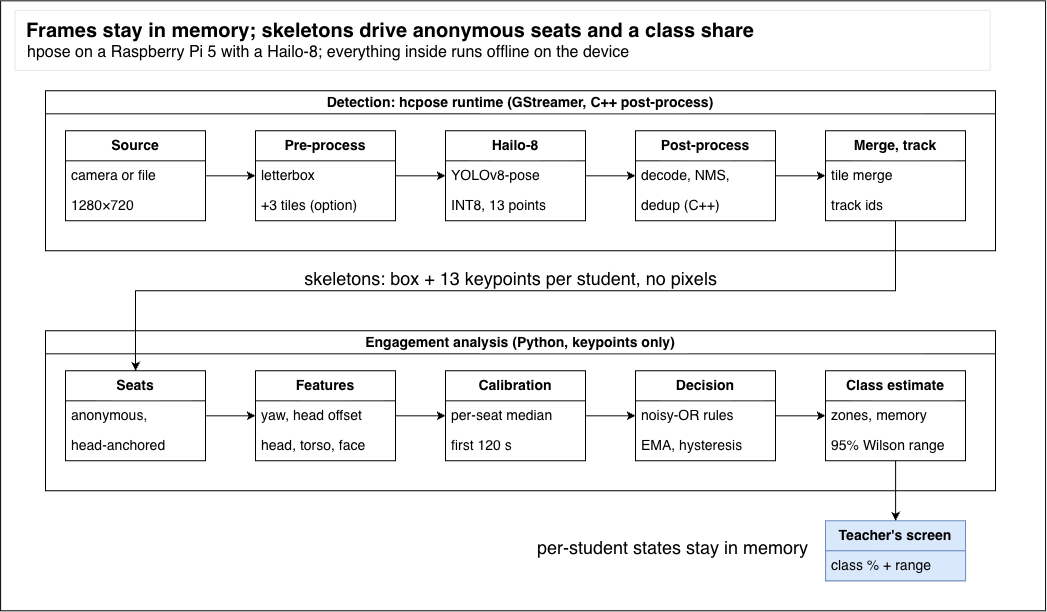
\includegraphics[width=1.0\textwidth]{figures/architecture.png}
\caption{Kiến trúc của hcpose: khung hình chỉ nằm trong bộ nhớ, các bộ khung xương dẫn tới các chỗ ngồi ẩn danh và một tỷ lệ cấp lớp}\label{fig:architecture-of-hcpose-frames-stay-in-me}
\end{figure}

Tệp khung xương (\texttt{-\/-save-json}) và video có chú thích (\texttt{-\/-output}) có thể được ghi ra ở điểm chuyển giữa hai giai đoạn để phục vụ phát triển và đánh giá. Cả hai đều tắt theo mặc định. Sơ đồ luồng dữ liệu dùng cho phân tích quyền riêng tư nằm ở chương 4.

\manualfigure{figures/manual/device}{Thiết bị}{Thiết bị: Raspberry Pi 5 với Hailo-8 AI HAT+ (26 TOPS), quạt tản nhiệt và camera.}{fig:device}

\section{Mô hình tư thế và biên dịch}

Các mô hình tư thế là mạng YOLOv8-pose ở ba kích thước n, s và m, dự đoán một lớp (người) và 13 điểm khóa phần thân trên: các điểm khóa COCO 0-12 \cite{b13}, từ mũi đến hông. Bàn học che khuất chân, nên các điểm phần thân dưới không mang thông tin. Các mô hình được huấn luyện trên COCO bằng Ultralytics \cite{b14}, trong kho mã đi kèm \texttt{hailo-custom-yolo-pose}\footnote{Mã huấn luyện và biên dịch: \url{https://github.com/LTH3ar/hailo-custom-yolo-pose}}, và được giữ cố định trong luận văn này.

\textbf{Huấn luyện.} Cả ba kích thước đều bắt đầu từ trọng số YOLOv8-pose đã huấn luyện trước trên COCO của Ultralytics, rồi được tinh chỉnh trên tập điểm khóa người COCO 2017: train2017 để huấn luyện, val2017 để kiểm định. Nhãn được chuyển đổi bằng \texttt{convert\_coco} của Ultralytics và cắt từ 17 xuống 13 điểm khóa. Thiết lập giống nhau cho mọi kích thước, trừ kích thước batch:

\begin{itemize}
\tightlist
\item
  100 epoch ở 640×640; batch 16 cho n và m, 32 cho s; seed 0, chế độ tất định, độ chính xác hỗn hợp.
\item
  \texttt{optimizer=auto}: Ultralytics tự chọn bộ tối ưu và tốc độ học. Tốc độ học trong log cho thấy 3 epoch khởi động, sau đó giảm tuyến tính xuống 1\% giá trị đỉnh vào epoch 100.
\item
  Trọng số hàm mất mát và tăng cường dữ liệu theo mặc định của Ultralytics: nhiễu HSV, scale 0.5, translate 0.1, và lật ngang với xác suất 0.5 kèm hoán đổi điểm khóa trái và phải. Mosaic được bật trừ 10 epoch cuối.
\end{itemize}

Việc huấn luyện chạy trên máy trạm của dự án (một NVIDIA RTX 3060) với phiên bản Ultralytics tháng 6/2026.

\begin{table}[htbp]\small
\caption{Huấn luyện ba mô hình tư thế}\label{tab:training-of-the-three-pose-models}
\begin{tabularx}{\textwidth}{*{4}{>{\raggedright\arraybackslash}X}}
\toprule
\textbf{Mô hình} & \textbf{Epoch tốt nhất} & \textbf{Thời gian huấn luyện (giờ)} & \textbf{Box mAP50-95 (log huấn luyện)} \\
\midrule
n & 100 & 43.1 & 0.527 \\
s & 99 & 42.4 & 0.584 \\
m & 96 & 89.9 & 0.619 \\
\bottomrule
\end{tabularx}
\end{table}

\textbf{Độ chính xác điểm khóa.} Trên COCO val2017, các mô hình đã huấn luyện đạt keypoint AP 0.470, 0.568 và 0.625 trên 13 điểm của chúng, thấp hơn 4-5 điểm so với các mô hình 17 điểm gốc trên cùng các điểm đó. Trên Hailo-8, lượng tử hóa INT8 làm n mất 5.3 điểm và m mất 6.8 điểm. HEF của s mất 30.8 điểm, nên bị loại khỏi mọi kết quả về độ chính xác.

\begin{table}[htbp]\small
\caption{Keypoint AP trên COCO val2017, 13 điểm khóa thân trên, dung sai COCO}\label{tab:keypoint-ap-on-coco-val2017-13-upper-bod}
\begin{tabularx}{\textwidth}{*{5}{>{\raggedright\arraybackslash}X}}
\toprule
\textbf{Mô hình} & \textbf{Mô hình 17 điểm gốc, trên 13 điểm} & \textbf{Mô hình 13 điểm đã huấn luyện (.pt)} & \textbf{HEF INT8 trên Hailo-8} & \textbf{Mất mát do INT8 (điểm AP)} \\
\midrule
n & 0.523 & 0.470 & 0.417 & −5.3 \\
s & 0.613 & 0.568 & 0.260 & −30.8 \\
m & 0.665 & 0.625 & 0.557 & −6.8 \\
\bottomrule
\end{tabularx}
\end{table}

Keypoint AP (OKS 0.50:0.95) trên 5.000 ảnh val2017, chấm bằng pycocotools \cite{b15} với dung sai theo từng điểm khóa của COCO. Mọi mô hình nhận cùng một ảnh letterbox 640×640. Để kiểm tra cách chấm, các mô hình gốc đạt 0.499, 0.594 và 0.645 trên đủ 17 điểm, chênh không quá 0.6 điểm so với các giá trị 50.4, 60.0 và 65.0 mà Ultralytics công bố.

\begin{itemize}
\tightlist
\item
  \textbf{Kích thước.} Trên Hailo-8, m hơn n 0.14 AP (0.557 so với 0.417), với độ trễ gấp 4.7 lần.
\item
  \textbf{Huấn luyện trên 13 điểm.} Phần lớn mức giảm 4-5 điểm nằm ở việc định vị chính xác các điểm trên khuôn mặt. Với cùng một dung sai rộng cho mọi điểm, khoảng cách thu hẹp còn 1.1-1.5 điểm.
\item
  \textbf{HEF của s.} Mô hình vẫn tìm được người (AP50 0.683) nhưng định vị điểm khóa kém (AP75 0.127). Trên các phát hiện được ghép cặp, sai số trung vị của điểm khóa là 4-9\% kích thước hộp, so với 2-3\% của HEF n và m, và mọi điểm đều bị lệch theo cùng một hướng. Mô hình n được biên dịch bằng cùng script mà không bị ảnh hưởng, nên lỗi nằm ở lần biên dịch này chứ không ở thiết lập: nguyên nhân là một lần lượng tử hóa thất bại (SNR đầu ra 4-11 dB). Tối ưu hóa lại với đúng các ảnh hiệu chỉnh đó cho AP 0.487, và năm lần biên dịch lại với các seed hiệu chỉnh khác nhau cho 0.508 ± 0.011. Mô hình s chỉ xuất hiện trong các kết quả về tốc độ.
\item
  \textbf{Điểm số trong log huấn luyện.} Keypoint mAP50-95 trong log (0.329, 0.376, 0.401) thấp hơn nhiều so với cùng các mô hình được pycocotools chấm với cùng một dung sai đồng nhất (0.579, 0.660, 0.706). Nguyên nhân là những người không có điểm khóa nào được gán nhãn trong 13 điểm. Họ chiếm 4.503 trên 10.777 người trong nhãn kiểm định (41.8\%). pycocotools bỏ qua họ, nhưng bộ kiểm định của Ultralytics tính họ là các mục tiêu không bao giờ ghép được. Khi loại những người này, chính bộ kiểm định của Ultralytics cho 0.555, 0.632 và 0.669, gần với số liệu của pycocotools. Vì vậy log đánh giá thấp độ chính xác điểm khóa, và các điểm số keypoint trong log không được dùng làm kết quả.
\end{itemize}

Để chạy trên Hailo-8, mỗi mô hình được lượng tử hóa INT8 và biên dịch bằng Hailo Dataflow Compiler thành một HEF:

\begin{itemize}
\tightlist
\item
  \textbf{Không có NMS trên chip.} Chín đầu ra thô của head được xuất làm nút cuối: phân bố hộp (DFL), điểm lớp và điểm khóa ở các stride 8, 16 và 32. Giải mã và NMS chạy trên CPU của máy chủ, giúp HEF không phụ thuộc vào số điểm khóa của mô hình.
\item
  \textbf{Sigmoid bên trong HEF.} Điểm lớp được đưa qua sigmoid ngay trong HEF. Runtime tự phát hiện điều này cho từng mô hình, qua đó sửa lỗi sigmoid hai lần trong mã cũ mà nó thay thế.
\end{itemize}

\begin{table}[htbp]\small
\caption{Thông lượng và độ trễ của các HEF INT8 khi chỉ chạy trên Hailo-8}\label{tab:throughput-and-latency-of-the-int8-hefs-}
\begin{tabularx}{\textwidth}{*{3}{>{\raggedright\arraybackslash}X}}
\toprule
\textbf{Mô hình} & \textbf{FPS trên Hailo-8} & \textbf{Độ trễ phần cứng (ms)} \\
\midrule
n & 131.5 & 5.7 \\
s & 69.5 & 11.9 \\
m & 31.5 & 26.7 \\
\bottomrule
\end{tabularx}
\end{table}

\textbf{Lượng tử hóa.} Trình biên dịch (Hailo Dataflow Compiler 3.33.1, Model Zoo 2.18) hiệu chỉnh khoảng giá trị INT8 trên 1.024 ảnh train2017 ngẫu nhiên đã đổi kích thước về 640×640. Mô hình n và s dùng chung một model script, còn m có script riêng. Cả hai script giữ ba trong chín lớp đầu ra ở 16 bit; theo thứ tự, đó là các đầu ra điểm khóa. Cả hai chạy bước tinh chỉnh sau lượng tử hóa của Hailo với tốc độ học 0.00015, và script n/s tắt thêm bước cân bằng trước lượng tử hóa.

\section{Runtime: hcpose}

hcpose chạy mọi HEF YOLOv8-pose trên Raspberry Pi 5. Khi khởi động, nó đọc từ HEF số điểm khóa, các stride, thứ tự tensor, kiểu dữ liệu đầu ra và hàm kích hoạt của điểm số, nên cùng một lệnh có thể chạy mô hình 13 điểm, mô hình 17 điểm gốc hoặc các mô hình khác.

\textbf{Engine.}

\begin{itemize}
\tightlist
\item
  \textbf{Engine GStreamer} (mặc định, cho chạy trực tiếp): nguồn camera hoặc tệp đưa vào \texttt{hailonet}. Một \texttt{hailofilter} C++ giải mã và hậu xử lý đầu ra, \texttt{hailotracker} gán mã theo dõi, và \texttt{hailooverlay} vẽ kết quả.
\item
  \textbf{Engine Python} (cho ảnh, gỡ lỗi và đánh giá): OpenCV và HailoRT với bộ giải mã NumPy.
\item hai bộ giải mã cho ra các phát hiện giống hệt nhau, được kiểm tra bằng các bài test trên đầu ra mô hình đã ghi lại.
\end{itemize}

\textbf{Hậu xử lý.}

\begin{itemize}
\tightlist
\item
  \textbf{Giải mã:} hộp DFL và điểm khóa được giải mã và ánh xạ ngược qua letterbox.
\item
  \textbf{NMS:} các ứng viên được sắp xếp theo điểm số trước. Mã kế thừa bỏ qua bước này, nên các chồng lấn được giải quyết theo thứ tự anchor.
\item
  \textbf{Loại bỏ khung xương trùng lặp:} sau NMS, một hộp bị loại khi nằm trong một hộp có điểm cao hơn và bộ khung xương khớp nhau: có ít nhất ba điểm khóa chung, khoảng cách trung bình nhỏ hơn 0.1 × √(diện tích hộp nhỏ hơn). YOLO-pose thường xuất một hộp chặt và một hộp lỏng cho cùng một học sinh, và NMS theo hộp giữ lại cả hai.
\end{itemize}

\textbf{Chia ô ảnh cho các hàng xa.} Với \texttt{-\/-tiles}, mô hình chạy thêm trên một hàng các ô gần vuông, chồng lấn nhau, phủ 60\% phía trên của khung hình (ba ô ở độ phân giải 1280×720).

\begin{itemize}
\tightlist
\item
  \textbf{Trong engine GStreamer:} một hàm cắt tùy biến đưa cho \texttt{hailocropper} toàn bộ khung hình cùng các ô. Một \texttt{hailofilter} thứ hai sau bộ gộp sẽ hợp nhất kết quả.
\item
  \textbf{Hợp nhất:} phát hiện trong các ô được ánh xạ về tọa độ khung hình, các phát hiện bị cắt bởi cạnh trong của ô bị loại, và các phát hiện trùng giữa các lượt được gộp theo IoU, hoặc theo quan hệ bao chứa kèm điểm khóa khớp nhau.
\item
  \textbf{Kiểm tra:} kết quả gộp bằng C++ trùng với kết quả gộp bằng Python trên 25 cảnh ngẫu nhiên.
\item
  \textbf{Chi phí:} chia ô ảnh làm khối lượng suy luận tăng gấp bốn.
\end{itemize}

\manualfigure{figures/manual/tiles}{Các ô ảnh}{Phát hiện trên video phòng thi khi không có (trái) và có (phải) ba ô phủ các hàng xa.}{fig:tiles}

\textbf{Đầu ra.}

\begin{itemize}
\tightlist
\item
  Cửa sổ có chú thích, hoặc chạy không giao diện.
\item
  Tùy chọn một video có chú thích (\texttt{-\/-output}), chỉ dùng khi phát triển.
\item
  Tùy chọn một tệp khung xương JSON-lines (\texttt{-\/-save-json}) chứa hộp và điểm khóa, không có điểm ảnh.
\end{itemize}

\manualfigure{figures/manual/displays}{Hai chế độ hiển thị}{Trái: chế độ phát triển với trạng thái từng học sinh (xanh lá: tập trung, đỏ: mất tập trung, trắng: đang hiệu chỉnh). Phải: chế độ dành cho giáo viên, chỉ có tỷ lệ của lớp và khoảng 95\%.}{fig:displays}

\section{Phân tích mức độ tập trung}

Bộ phân tích biến các bộ khung xương của mỗi khung hình thành trạng thái \textbf{tập trung}, \textbf{mất tập trung} hoặc \textbf{không xác định} cho từng học sinh, cùng một tỷ lệ cấp lớp kèm khoảng. Nó chỉ làm việc trên điểm khóa và có thể chạy lại một tệp khung xương đã lưu (\texttt{hcpose\ analyze}) với bất kỳ thiết lập nào.

\textbf{Chỗ ngồi.} Học sinh được theo dõi dưới dạng các chỗ ngồi ẩn danh, ghép giữa các khung hình theo điểm giữa cạnh trên của hộp (phần đầu). Phần đầu giữ nguyên vị trí khi học sinh nghiêng người hay quay lại, trong khi tâm hộp nhảy đi. Một chỗ ngồi chỉ được tính vào lớp khi nó đang hiện diện và được thấy ổn định.

\textbf{Đặc trưng}, chuẩn hóa theo bề rộng vai:

\begin{itemize}
\tightlist
\item
  \textbf{Hai thước đo góc quay đầu.} Góc yaw dựa trên tai: vị trí mũi giữa hai tai. Độ lệch đầu: vị trí mũi so với trung điểm hai vai, vẫn hoạt động khi nhìn nghiêng.
\item
  \textbf{Độ cao đầu} so với đường vai.
\item
  \textbf{Tỷ lệ thân}, giảm khi cơ thể xoay.
\item
  \textbf{Khuôn mặt bị khuất} trong khi vẫn thấy vai.
\item
  \textbf{Giơ tay}, và \textbf{tay đưa lên mặt}.
\end{itemize}

\textbf{Hiệu chỉnh theo từng chỗ ngồi.}

\begin{itemize}
\tightlist
\item
  Mỗi chỗ ngồi học tư thế chú ý của riêng nó, là trung vị của 120 giây quan sát dùng được đầu tiên. Trước đó, hệ thống dùng trung vị từng phần và trung vị của cả phòng.
\item
  Giá trị gốc về yaw và độ lệch đầu của chỗ ngồi được giữ trong phạm vi 0.3 và 0.15 so với giá trị của cả phòng, để một học sinh nhìn đi chỗ khác trong lúc hiệu chỉnh không học ``quay đi'' thành trạng thái bình thường.
\item
  \texttt{-\/-camera-position} (trái, giữa, phải) đặt giá trị tiên nghiệm cho hướng chú ý của cả phòng.
\end{itemize}

\textbf{Quyết định.} Mỗi dấu hiệu là một hàm dốc từ ``bình thường'' đến ``rõ ràng lệch'' so với giá trị gốc của chỗ ngồi. Các dấu hiệu được kết hợp bằng noisy-OR, nên các dấu hiệu yếu chỉ có tác dụng khi đi cùng một dấu hiệu khác: xoay người và tay đưa lên mặt không bao giờ tự mình đánh dấu một học sinh, còn cúi đầu (viết bài trông cũng như vậy) chỉ khi đầu hạ thấp hơn hẳn mức bình thường của chỗ ngồi:

\begin{equation}
s = 1 - \prod_{c} \left(1 - w_c \, r_c\right)
\end{equation}

Trong đó r\_c là giá trị hàm dốc của dấu hiệu c và w\_c là trọng số của nó. Giơ tay đặt điểm số về 0. Trọng số mặc định: quay đầu 1.0, khuôn mặt bị khuất 0.9, cúi đầu 0.7, xoay người 0.5, tay đưa lên mặt 0.4. Các bộ phân loại học máy (cây quyết định, hồi quy logistic, MLP) có thể thay thế noisy-OR, nhưng tắt theo mặc định (chương 4).

\textbf{Làm trơn.} Điểm số được làm trơn bằng trung bình trượt hàm mũ (τ = 1 s) và chuyển trạng thái có trễ (hysteresis):

\begin{itemize}
\tightlist
\item
  \textbf{sang mất tập trung:} trên 0.6 trong 2.5 s
\item
  \textbf{trở lại tập trung:} dưới 0.4 trong 1.5 s
\item
  \textbf{không xác định:} không có điểm khóa dùng được trong 2 s
\end{itemize}

Nhờ vậy một cái liếc mắt ngắn không làm đổi trạng thái của học sinh.

\textbf{Ước lượng cấp lớp.}

\begin{itemize}
\tightlist
\item
  Chỗ ngồi giữ trạng thái cuối cùng trong 15 s sau lần cuối được thấy.
\item
  Chúng được chia thành các vùng gần, giữa và xa theo chiều cao trong ảnh, và mỗi vùng được gán trọng số theo số chỗ ngồi.
\item
  Tỷ lệ của lớp đi kèm khoảng Wilson 95\% \cite{b16} quanh giá trị hiển thị (đã làm trơn). Khoảng này chỉ được thu hẹp bằng hệ số hiệu chỉnh tổng thể hữu hạn khi biết sĩ số thực (\texttt{-\/-class-size}).
\item
  Trên màn hình: ``43\% mất tập trung (20-65\%) \textbar{} 14 trên \textasciitilde30 học sinh''.
\end{itemize}

\section{Cấu hình, kiểm thử và khả năng tái lập}

\textbf{Cấu hình.} Mọi ngưỡng, trọng số và tùy chọn đều là một thiết lập trong \texttt{configs/engagement.yaml} hoặc một cờ dòng lệnh:

\begin{itemize}
\tightlist
\item
  vị trí camera
\item
  chế độ hiển thị (từng học sinh, cả lớp, cả hai hoặc không)
\item
  sĩ số lớp
\item
  tệp hiệu chỉnh
\item
  bộ phân loại
\item
  chia ô ảnh
\end{itemize}

Một tệp YAML đi kèm mỗi mô hình đặt các ngưỡng phát hiện và tên điểm khóa.

\textbf{Kiểm thử.} 44 bài test tự động bao gồm:

\begin{itemize}
\tightlist
\item
  cả hai bộ giải mã, so với đầu ra HEF đã ghi và cách giải mã của chính Ultralytics
\item
  phép ánh xạ letterbox và hợp nhất ô ảnh bằng C++, so với Python
\item
  bước loại bỏ trùng lặp
\item
  logic đánh giá mức độ tập trung trên các lớp học tổng hợp: hiệu chỉnh, liếc mắt, khung hình bị thiếu, đếm chỗ ngồi, khoảng tin cậy, thước đo độ lệch đầu
\item
  bộ chấm điểm buổi dàn dựng trên một buổi tổng hợp có đáp án biết trước
\end{itemize}

\textbf{Khả năng tái lập.} Kết quả và các công cụ tạo ra chúng nằm trong kho mã:

\begin{itemize}
\tightlist
\item
  tệp khung xương từ Pi
\item
  log trên thiết bị biên
\item
  nhãn do người gán
\item
  kịch bản các buổi dàn dựng
\item
  các lần quét ngưỡng
\end{itemize}

Mọi phân tích đều có thể chạy lại từ các bộ khung xương đã lưu mà không cần video từ camera. Phiên bản được đánh giá được gắn tag \texttt{v1.0.3}.
